
\section[Methodology]{Methodology: Policy Learning Framework for Replay Scheduling}\label{paperD:sec:methodology}

In this section, we present an RL-based framework for learning replay scheduling policies. We focus on learning a general policy that can be applied in any CL scenario to mitigate catastrophic forgetting to avoid re-training the policy for every new CL dataset. 
Our intuition is that there may exist general patterns regarding replay scheduling, e.g., that tasks that are harder or have been forgotten should be replayed more often. We aim to implicitly explore such task properties by using the task performances of the CL network as states for the policy to select which tasks to replay. Representing the states with task performances also enables transferring the learned policy to reduce forgetting in unseen CL environments. For example, we could apply a learned policy in user personalization scenarios, where an image classifier learns continually to recognize various objects in environments of different people. 
Next, we present our modeling approach for learning the replay scheduling policies using RL. 

\begin{figure}[t]
	\centering
	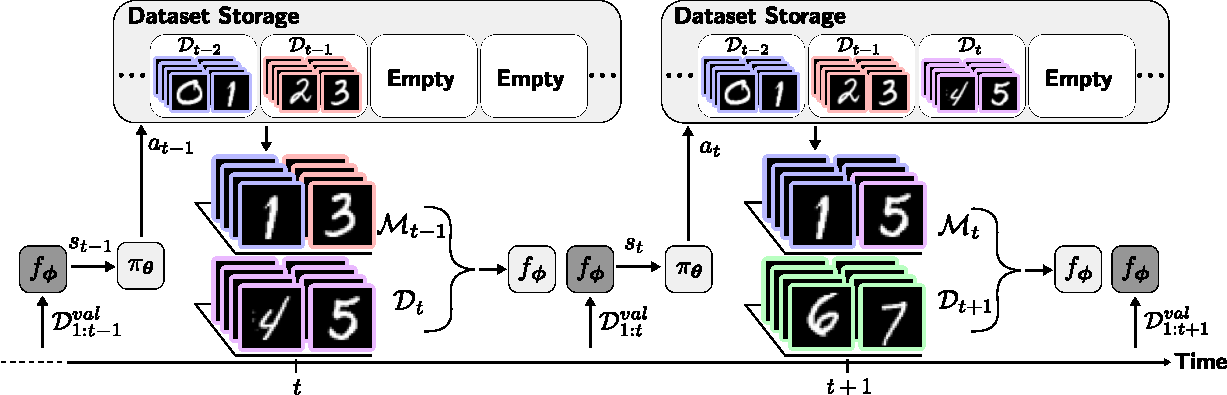
\includegraphics[width=0.95\textwidth]{Chapter1/figures/testing_size2.pdf}
	\caption{Illustration of the procedure of the proposed RL-based framework in a CL environment with Split MNIST. The goal is to mitigate catastrophic forgetting in the classifier $f_{\vphi}$ by composing replay memories $\gM$ with the replay scheduling policy $\pi_{\vtheta}$. The policy selects action $a$ determining which tasks to replay given the state $s$ represented as the validation task performances of $f_{\vphi}$. The colored border on the MNIST images indicates which task the data comes from. The classifier $f_{\vphi}$ is in evaluation mode when darker-shaded color over the box is used. %Pipeline of our proposed RL-based framework. 
	}
	\label{fig:rl_framework_pipeline}
	\vspace{-2mm}
\end{figure}

\vspace{-3mm}
\paragraph{CL Environment.} We model the CL environments as Markov Decision Processes~\citeD{D:bellman1957markovian} (MDPs) where each MDP is represented as a tuple $E_i = (\gS_i, \gA, P_i, R_i, \mu_i, \gamma)$ consisting of the state space $\gS_i$, action space $\gA$, state transition probability $P_i(s' | s, a)$, reward function $R_i(s, a)$, initial state distribution $\mu_i(s_1)$, and discount factor $\gamma$. 
Each environment $E_i$ contains a network $f_{\vphi}$ and task datasets $\gD_{1:T}$ where the $t$-th dataset is learned at time step $t$.  
The state $s_t$ is defined as the task accuracies $A_{t,1:t}$ evaluated at task $t$, such that $s_t = [A_{t, 1}, ..., A_{t, t}, 0, ..., 0]$ where zero-padding is used on future tasks. We obtain the states by evaluating the classifier on the validation datasets to avoid overfitting the policy to the training data.
We use the same action space as constructed in Klasson \etal~\citeD{D:klasson2021learn}, such that $a_t \in \gA$ corresponds to a task proportion $\vp_t$ used for sampling the replay memory $\gM_t$. 
The state transition distribution $P_i(s' | s, a)$ represents the dynamics of the environment, which depend on the initialization of $f_{\vphi}$ and the task order in $\gD_{1:T}$. 
We use a dense reward defined as the average validation accuracies at task $t$, i.e., $r_{t} = \frac{1}{t}\sum_{i=1}^{t} A_{t, i}^{(val)}$, to ease exploration in the action space. The goal for the agent is to maximize the rewards during an episode.


\vspace{-3mm}
\paragraph{Policy Training and Evaluation.} Figure \ref{fig:rl_framework_pipeline} shows an illustration of this procedure for using the learned replay scheduling policy in a CL environment with the Split MNIST dataset~\citeD{D:zenke2017continual}. The seen CL datasets are placed in the dataset storage to use for sampling replay memories given the actions from the policy $\pi_{\vtheta}$ for mitigating catastrophic forgetting at each time step. The policy interacts with the CL environments by selecting which tasks the network $f_{\vphi}$ should replay to mitigate catastrophic forgetting. The state $s_t$ is obtained by evaluating $f_{\vphi}$ on the validation sets $\gD_{1:t}^{(val)}$ after learning task $t$. The action $a_t$ is selected under the policy $\pi_{\vtheta}(a | s_t)$, parameterized by $\vtheta$, which is converted into the task proportion $\vp_t$ for sampling the replay memory $\gM_t$ from the historical datasets. The network $f_{\vphi}$ is trained on task $t+1$ while replaying $\gM_t$, and we obtain the reward $r_{t+1}$ and the next state $s_{t+1}$ by evaluating $f_{\vphi}$ on the validation sets $\gD_{1:t+1}^{(val)}$. The collected transitions $(s_t, a_t, r_{t+1}, s_{t+1})$ are used for updating the policy, and a new episode starts after $f_{\vphi}$ has learned the final task $T$. We let the policy interact with multiple training environments $\gE^{(train)} = \{E_i\}_{i=1}^{K}$ sampled from a distribution of CL environments, i.e., $E_i \sim p(E)$. To generate diverse CL environments, we let each $E_i$ have different network initializations of $f_{\vphi}$ and task orders in the datasets. 
Our goal is to learn a general replay scheduling policy that can be applied in new CL environments to mitigate catastrophic forgetting. Hence, in Section \ref{paperD:sec:experiments}, we evaluate the policy in CL environments with new task orders or datasets unseen during training. The policy is applied for only a single CL episode without additional training in the test environment. 

\vspace{-3mm}
\paragraph{Architectures for RL algorithms.}
The input layer to the RL policy networks has size $T-1$ where each unit is inputting the task performances since the states are represented by the validation accuracies $s_t = [A_{t, 1}^{(val)}, ..., A_{t, t}^{(val)}, 0, ..., 0]$. The current task can therefore be determined by the number of non-zero state inputs. For DQN and A2C, we use a Categorical policy where the output layer has 35 units representing the possible actions at $T=5$ in the discrete action space (see Klasson \etal~\citeD{D:klasson2021learn}). We use action masking on the output units based on the task number to prevent the network from selecting invalid actions for constructing the replay memory at the current task. 
For SAC, we take inspiration from Tian \etal~\citeD{D:tian2022prescriptive} and use a Dirichlet policy for representing the task proportions in a continuous action space, where the actions are constrained by $\sum_{i=1}^{t-1} a_i = 1$ where $a_i \geq 0$. The continuous action space has $T-1$ dimensions, where each dimension represents the task proportion to use for filling the replay memory with samples from the corresponding task. We use zero-masking on the Dirichlet concentration parameters based on the current task to prevent invalid actions. In the experiments (Section \ref{paperD:sec:experiments}), we select the closest action measured in Euclidean distance from the discrete action space as the executed action for SAC to establish fair comparison to DQN and A2C. 
%The DQN is a 2-layer MLP with 512 hidden units and ReLU activations. For A2C, we use separate networks for parameterizing the policy and the value function, where both networks are 2-layer MLPs with 64 hidden units of Tanh activations. 


\begin{comment}
In this section, we present an RL-based framework for learning replay scheduling policies that generalize across different CL scenarios. Our intuition is that there may exist general patterns regarding the replay scheduling, e.g., tasks that are harder or have been forgotten should be replayed more often. Moreover, the policy may non-trivially take task properties into consideration. Therefore, we aim to learn policies that select which tasks to replay from states representing the current task performance in the CL environments. The policy can then be applied for mitigating catastrophic forgetting in new CL scenarios. 


The CL environments are modeled using MDPs represented as tuples $E_i = (\gS_i, \gA, P_i, R_i, \mu_i, \gamma)$ sampled from a distribution of environments, such that $E_i \sim p(E)$ for $i=1, ..., K$. 
%We model the CL environments with MDPs represented by tuples $E_i = (\gS_i, \gA, P_i, R_i, \mu_i, \gamma)$ sampled from a distribution of CL environments, such that $E_i \sim p(E)$ for $i=1, ..., K$. 
We let the policy interact with a fixed set of environments $\gE^{(train)} = \{E_1, \dots, E_K\}$ sampled from the distribution $p(E)$ for training. 
Each environment $E_i$ contains of network $f_{\vphi}$ and $T$ datasets $\gD_{1:T}$ where the $t$-th dataset is learned at time step $t$. To generate diverse CL environments, we get environments with different network initializations of $f_{\vphi}$ and shuffled task orders in the dataset when we sample environments from $p(E)$. 
We define the state $s_t$ of the environment as the validation accuracies $A_{t, 1:t}^{val}$ on each seen task $1, ..., t$ from $f_{\vphi}$ at task $t$, i.e., $s_t = [A_{t, 1}, ..., A_{t, t}, 0, ..., 0]$, where we use zero-padding on future tasks. The action space $\gA$ is constructed as in Klasson \etal~\citeD{D:klasson2021learn}. 
%as described in Appendix \ref{paperD:app:action_space}, 
such that the $a_t \in \gA$ corresponds to a task proportion $\vp_t$ used for sampling the replay memory $\gM_t$. We use a dense reward based on the average validation accuracies at task $t$, i.e., $r_{t} = \frac{1}{t}\sum_{i=1}^{t} A_{t, i}^{val}$. The state transition distribution $P_i(s' | s, a)$ represents the dynamics of the environment, which depend on the initialization of $f_{\vphi}$ and also the task order in the dataset. 



The procedure for training the policy goes as follows: 
The state $s_{t}$ is obtained by evaluating the network $f_{\vphi}$ on the validation sets $\gD_{1:t}^{val}$ after learning the $t$-th task from $\gD_t^{(train)}$. Action $a_{t}$ is selected under the policy $\pi_{\vtheta}(a | s_{t})$ parameterized by $\vtheta$. The action is converted into task proportion $\vp_t$ for sampling the replay memory $\gM_{t}$ from the historical datasets $\gD_{1:t}^{train}$. 
We then train classifier $f_{\vphi}$ with $\gD_{t+1}^{(train)}$ and $\gM_{t}$, and obtain the reward $r_{t+1}$ and the next state $s_{t+1}$ by evaluating $f_{\vphi}$ on the validation sets $\gD_{1:t}^{val}$. The collected transitions $(s_t, a_t, r_{t+1}, s_{t+1})$ are used for updating the policy. This procedure is followed until the final task $T$ after which we start a new episode. %for collecting experience.   
Figure \ref{fig:rl_framework_pipeline} shows an illustration of this procedure for using the learned replay scheduling policy in a CL environment with the Split MNIST dataset~\citeD{D:zenke2017continual}. The seen datasets are placed in the dataset storage to use for sampling replay memories given the actions from the policy $\pi_{\vtheta}$ for mitigating catastrophic forgetting at each time step.

We evaluate the learned policy by applying it to mitigate catastrophic forgetting in new CL environments at test time. To foster generalization across environments, we train the policy on multiple environments with different dynamics, e.g., task orders and datasets, to learn from diverse sets of training data. The goal for the agent is to maximize the sum of rewards in each training environment. %We evaluate the policy by using it for selecting which tasks to replay in new CL environments. 
At test time, the policy is applied on new CL classifiers and datasets in the test environments without added computational cost nor experience collection. In Section \ref{paperD:sec:experiments}, we test the policies generalization capability to new CL environments where the task orders and datasets are unseen during training.

\end{comment}

